\documentclass{exam}

\usepackage{fullpage}
\usepackage{enumerate}
\usepackage{siunitx} 
\usepackage{graphicx}
\usepackage[fleqn]{amsmath}
\usepackage{cancel}
\usepackage{polynom}
\usepackage{float}
\usepackage{mdwlist}
\usepackage{booktabs}
\usepackage{cancel}
\usepackage{polynom}
\usepackage{caption}

\newcommand{\degree}{\ensuremath{^\circ}} 
\everymath{\displaystyle}

% \begin{figure}[H]
%   \centering
%   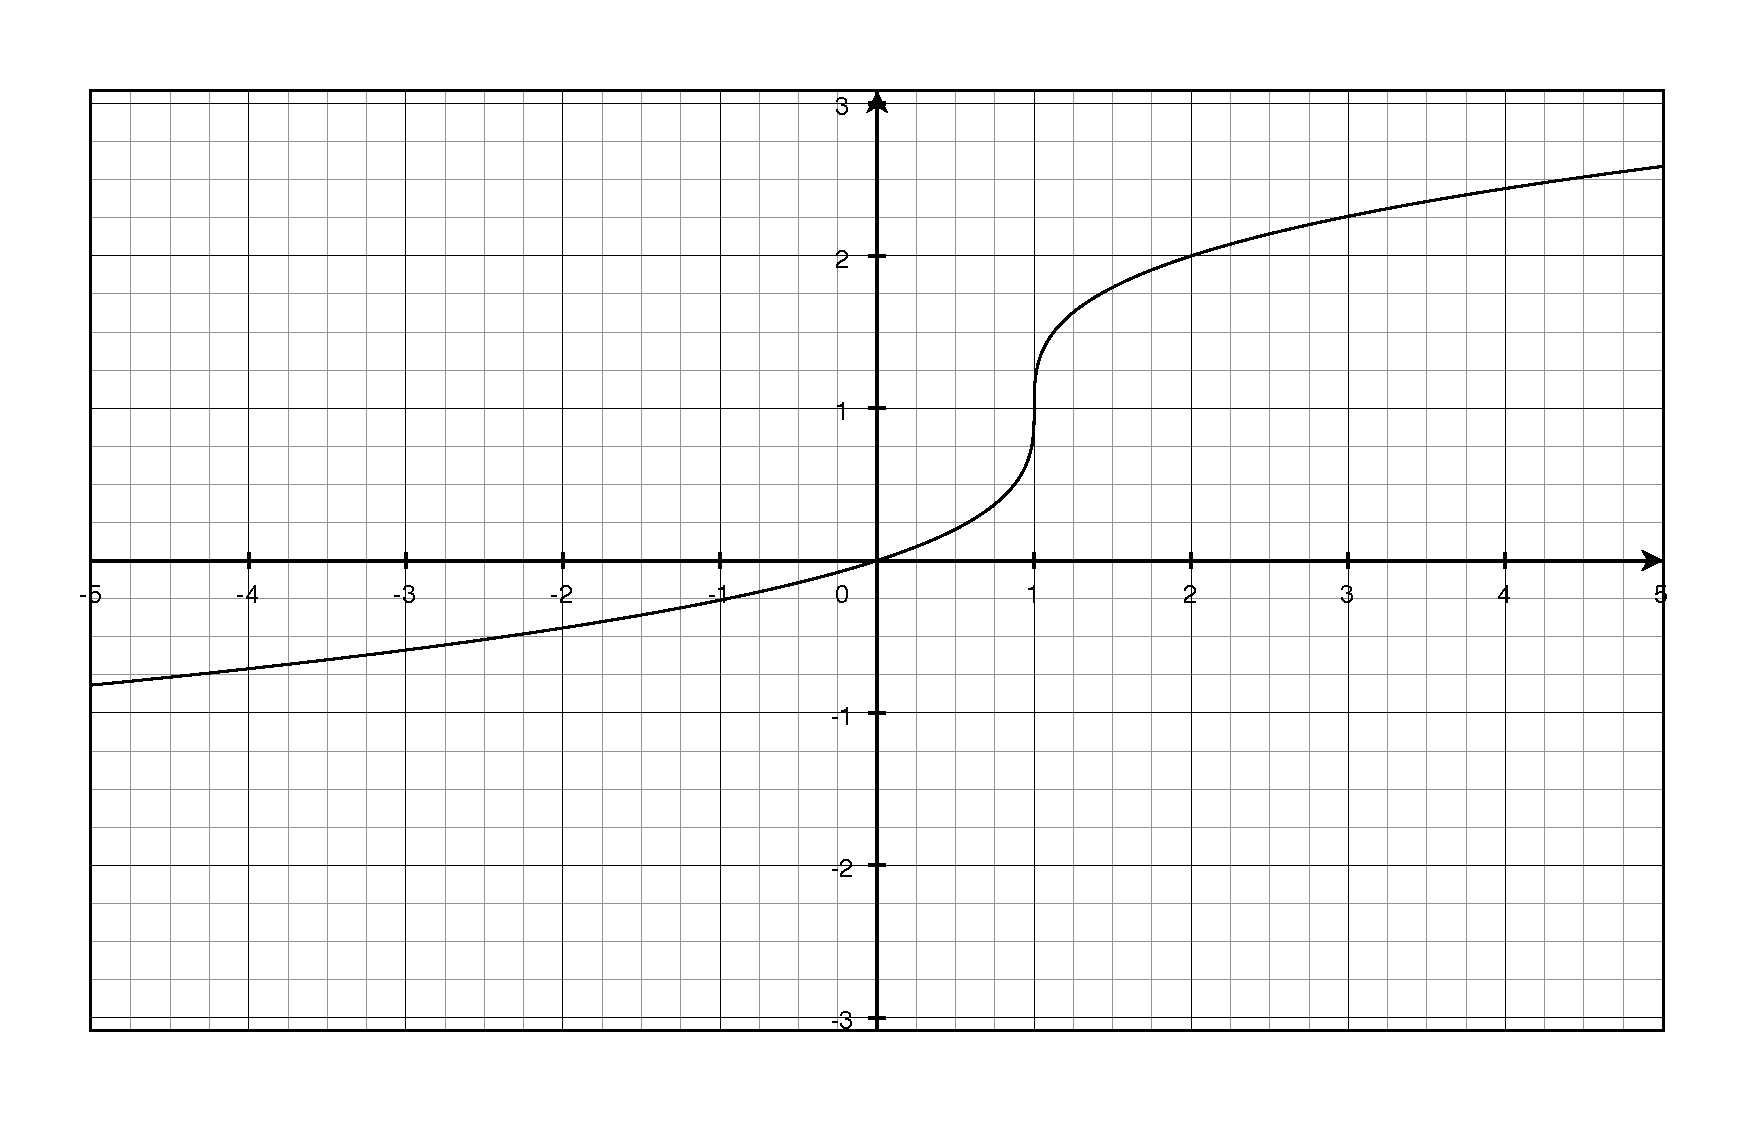
\includegraphics[scale=.3]{question7.eps}
%   \caption*{Question 7}
% \end{figure}

% \begin{tabular}{cc}
% \toprule
% period & amplitude \\
% \midrule
%   $\pi$ & $2$ \\
% \bottomrule
% \end{tabular}

\printanswers

\ifprintanswers 
\usepackage{2in1, lscape} 
\fi

\title{Math 263a \\ Homework Six}
\date{February 29, 2012 \\ Leap Day}

\begin{document}

\maketitle

\section{Homework}

\begin{itemize*}
  \item Read Section 3.3
  \item pp 121-122: 1-15, 21-25, 36-40, 49-50, 53
\end{itemize*}

\section{Extra Credit}

Page 122, problem 56

\ifprintanswers

Let's call the point where she shuts off the engines $(x_0, y_0)$

The slope of the tangent line is the derivative, or $y' = 2x$.  The slope of the tangent line at the engine shutoff
point is $2x_0$.  We need a line with this slope that passes through the point $(4, 15)$.  The equation for this line,
in terms of $x_0$ is:
\begin{align*}
  y - 15 &= 2x_0(x - 4) \\
  y &= 2x_0 x - 8x_0 + 15 \\
\end{align*}
The line also has to pass through the the engine shutoff point which happens at $y = x_0^2$.  We can set the two
equations equal to each other at this point to find $x_0$:
\begin{align*}
  2x_0^2 - 8x_0 + 15 &= x_0^2 \\
  x_0^2 - 8x_0 + 15 &= 0 \\
  (x_0 - 3)(x_0 - 5) &= 0 \\
\end{align*}
It looks like she could shut the engine off at either $x_0 = 3$ or $x_0 = 5$.  But since she is moving from left to right, she must shut her engines off when $x = 3$.  When $x = 5$, she will already have passed the target of $(4, 15)$ and will have to travel backwards along the tangent line to get there.

\begin{figure}[H]
  \centering
  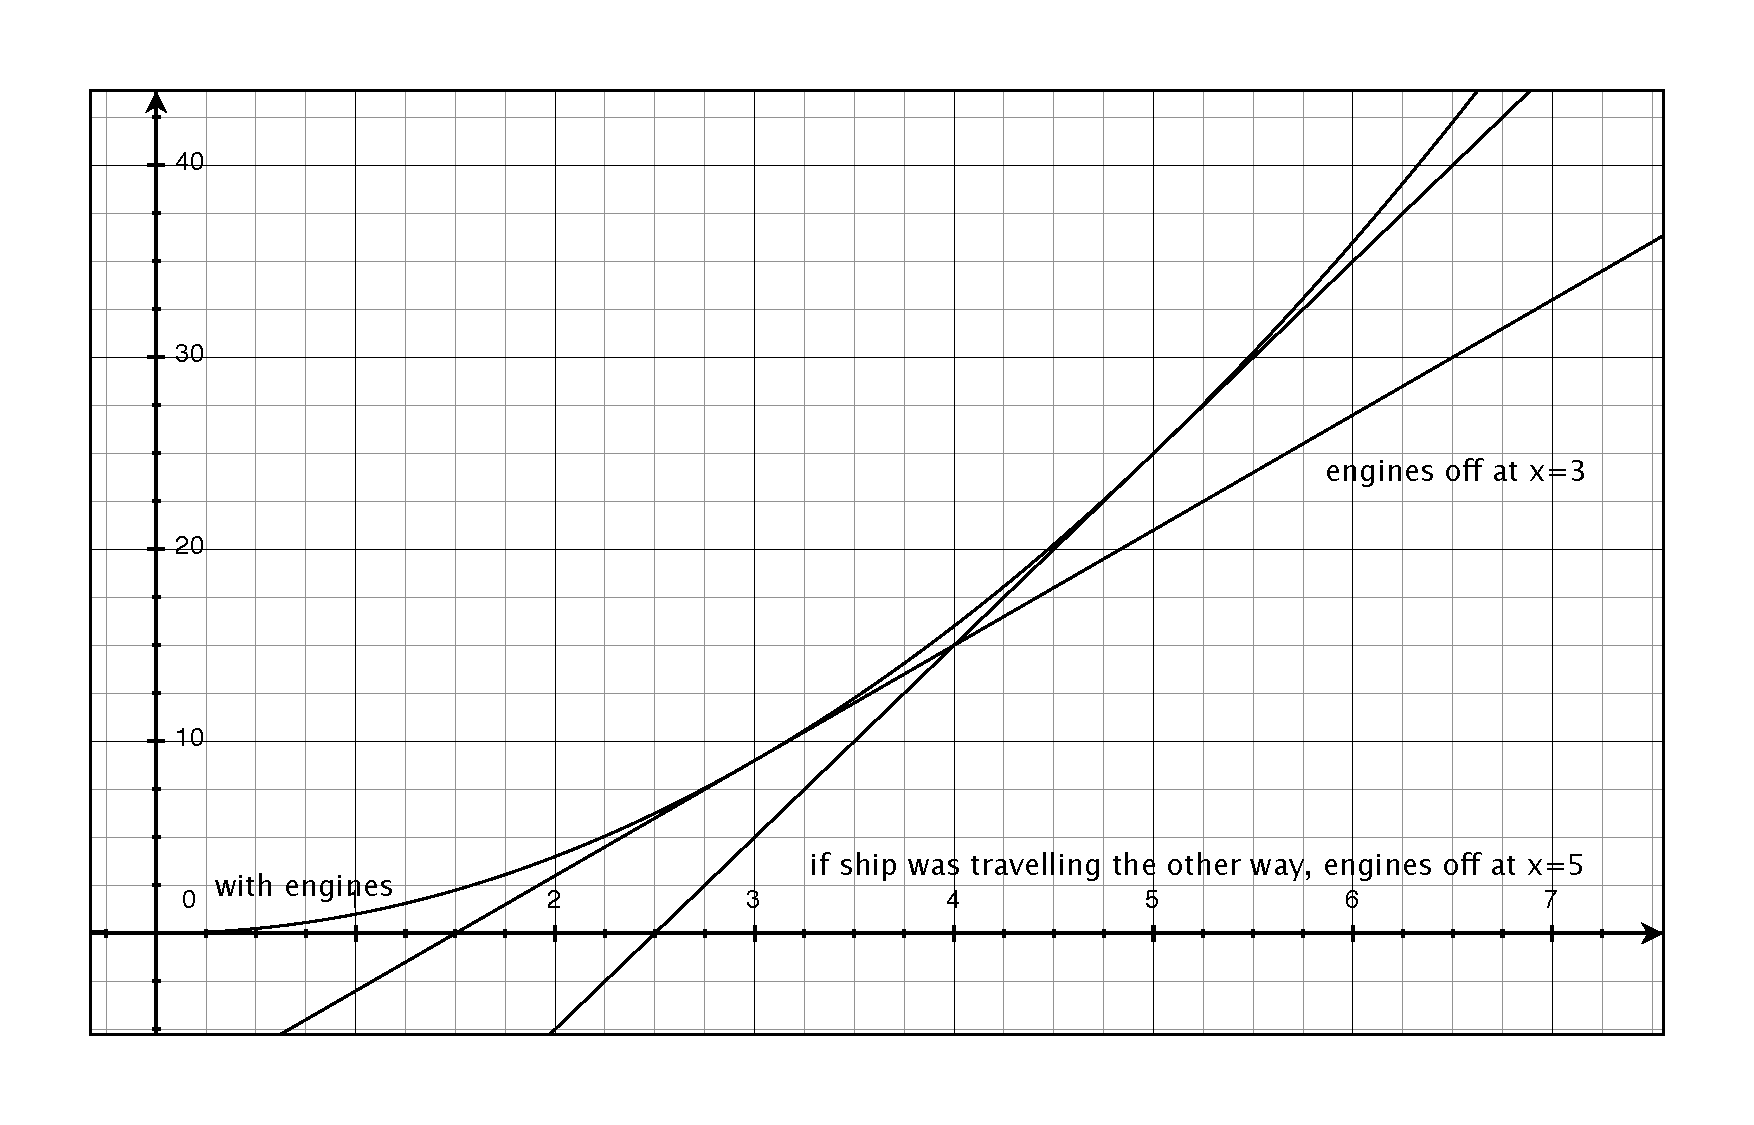
\includegraphics[scale=.3]{extra_credit.eps}
  \caption*{Extra Credit}
\end{figure}

\pagebreak

\section{Homework}

\begin{description}
\item[1]
\begin{align*}
  y &= 2x^2 \\
  y'&= 4x \\
\end{align*}

\item[2]
\begin{align*}
  y &= 3x^3 \\
  y'&= 9x^2 \\
\end{align*}

\item[3]
\begin{align*}
  y &= \pi x \\
  y'&= \pi \\
\end{align*}

\item[4]
\begin{align*}
  y &= \pi x^3 \\
  y'&= 3 \pi x^2 \\
\end{align*}

\item[5]
\begin{align*}
  y &= 2x^{-2} \\
  y'&= -4 x^{-3} \\
\end{align*}

\item[6]
\begin{align*}
  y &= -3 x^{-4} \\
  y'&= 12x^{-5} \\
\end{align*}

\item[7]
\begin{align*}
  y &= \frac{\pi}{x} \\
  y'&= - \frac{\pi}{x^2} \\
\end{align*}

\item[8]
\begin{align*}
  y &= \frac{\alpha}{x^3} \\
  y &= \alpha x^{-3} \\
  y' &= -3 \alpha x^{-4} \\
\end{align*}

\item[9]
\begin{align*}
  y &= \frac{100}{x^5} \\
  y &= 100 x^{-5} \\
  y' &= -500 x^{-6} \\
\end{align*}

\item[10]
\begin{align*}
  y &= \frac{3 \alpha}{4 x^5} \\
  y &= \frac{3 \alpha}{4} x^{-5} \\
  y' &= -\frac{15 \alpha}{4} x^{-6} \\
\end{align*}

\item[11]
\begin{align*}
  y &= x^2 + 2x \\
  y'&= 2x + 2 \\
\end{align*}

\item[12]
\begin{align*}
  y &= 3x^4 + x^3 \\
  y'&= 12x^3 + 3x^2 \\
\end{align*}

\item[13]
\begin{align*}
  y &= x^4 + x^3 + x^2 + x + 1 \\
  y' &= 4x^3 + 3x^2 + 2x + 1 \\
\end{align*}

\item[14]
\begin{align*}
  y &= 3x^4 - 2x^3 - 5x^2 + \pi x + \pi^2 \\
  y' &= 12x^3 - 6x^2 - 10x + \pi \\
\end{align*}

\item[15]
\begin{align*}
  y &= \pi x^7 - 2x^5 - 5x^{-2} \\
  y' &= 7 \pi x^6 - 10x^4 + 10x^{-3} \\
\end{align*}

\item[21]
\begin{align*}
  y  &= \frac{1}{2x} + 2x \\
  y' &= - \frac{2}{4x^2} + 2 \\
     &= - \frac{1}{2x^2} + 2 \\
\end{align*}

\item[22]
\begin{align*}
  y  &= \frac{2}{3x} - \frac{2}{3} \\
  y' &= - \frac{6}{9x^2} \\
     &= - \frac{2}{3x^2} \\
\end{align*}

\item[23]
\begin{align*}
  y  &= x(x^2 + 1) \\
  y' &= x(2x) + (x^2 + 1)(1) \\
     &= 2x^2 + x^2 + 1 \\
     &= 3x^2 + 1 \\
\end{align*}
or:
\begin{align*}
  y  &= x(x^2 + 1) \\
     &= x^3 + x\\
  y' &= 3x^2 + 1 \\
\end{align*}

\item[24]
\begin{align*}
  y  &= 3x(x^3 - 1) \\
  y' &= (3x)(3x^2) + (x^3 - 1)(3) \\
     &= 9x^3 + 3x^3 - 3 \\
     &= 12x^3 - 3 \\
\end{align*}
or:
\begin{align*}
  y  &= 3x(x^3 - 1) \\
     &= 3x^4 - 3x \\
  y' &= 12x^3 - 3 \\
\end{align*}

\item[25]
\begin{align*}
  y &= (2x+1)^2 \\
    &= (2x+1)(2x + 1) \\
  y' &= (2x + 1)(2)  + (2x + 1)(2) \\
     &= (4) (2x + 1) \\
     &= 8x + 4 \\
\end{align*}

\item[36]
\begin{align*}
  y  &= \frac{4}{2x^3 - 3x} \\
  y' &= \frac{-4(6x^2 - 3)}{(2x^3 - 3x)^2} \\
     &= \frac{-24x^2 + 12}{(2x^3 - 3x)^2} \\
\end{align*}

\item[37]
\begin{align*}
  y  &= \frac{x-1}{x+1} \\
  y' &= \frac{(x+1)(1) - (x-1)(1)}{(x + 1)^2} \\
     &= \frac{x+1 - x + 1}{(x+1)^2} \\
     &= \frac{2}{(x+1)^2} \\
\end{align*}

\item[38]
\begin{align*}
  y  &= \frac{2x-1}{x-1} \\
  y' &= \frac{(x-1)(2) - (2x-1)(1)}{(x - 1)^2} \\
     &= \frac{2x - 2 - 2x + 1}{(x-1)^2} \\
     &= \frac{-1}{(x-1)^2} \\
\end{align*}

\item[39]
\begin{align*}
  y  &= \frac{2x^2 - 1}{3x + 5} \\
  y' &= \frac{(3x + 5)(4x) - (2x^2 - 1)(3)}{(3x + 5)^2} \\
     &= \frac{12x^2 + 20x - 6x^2 +3}{(3x + 5)^2} \\
     &= \frac{6x^2 + 20x +3}{(3x + 5)^2} \\
\end{align*}

\item[40]
\begin{align*}
  y  &= \frac{5x - 4}{3x^2 + 1} \\
  y' &= \frac{(3x^2 + 1)(5) - (5x - 4)(6x)}{(3x^2 + 1)^2} \\
     &= \frac{15x^2 + 5 - 30x^2 + 24x)}{(3x^2 + 1)^2} \\
     &= \frac{-15x^2 - 24x + 5}{(3x^2 + 1)^2} \\
\end{align*}

\item[49]
\begin{align*}
  y  &= x^2 - 2x + 2 \\
  y' &= 2x - 2 \\
\end{align*}
The slope at $(1, 1)$ is $y'(1) = 2 - 2 = 0$

We need a line with slope 0 passing through point $(1, 1)$, which is just the line $y = 1$.

\item[50]
\begin{align*}
  y  &= \frac{1}{x^2 + 4} \\
  y' &= - \frac{2x}{(x^2 + 4)^2} \\
  \\
  y'(1) &= -\frac{2}{(1 + 4)^2} \\
     &= -\frac{2}{25} \\
\end{align*}

We need a line with slope $- \frac{2}{25}$ passing through point $\left(1, \frac{1}{5} \right)$:
\begin{align*}
  y - \frac{1}{5} &= - \frac{2}{25} (x - 1) \\
  y - \frac{1}{5} &= - \frac{2x}{25} + \frac{2}{25} \\
  y &= - \frac{2x}{25} + \frac{7}{25} \\
\end{align*}

\item[53]
\begin{align*}
  s(t) &= -16t^2 + 40t + 100 \\
  v(t) &= -32t + 40 \\
\end{align*}

\begin{enumerate}[a]
\item
\[
  v(2) = -64 + 40 = -24
\]

\item
\begin{align*}
  -32t + 40 &= 0 \\
  -32t      &= -40 \\
  t         &= 1.25 \text{ s} \\
\end{align*}

\end{enumerate}
\end{description}

\else

\vspace{10 cm}

% {\em People like us, who believe in physics, know that the distinction between past, present, and future is only a
%   stubbornly persistent illusion. (Einstein) }

% {\em I may be as woefully wrong as Humphrey Belcher who thought who believed the time was ripe for a cheese cauldron.}

{\em If those in charge of our society---politicians, corporate executives, and owners of press and television---can
  dominate our ideas, they will be secure in their power. They will not need soldiers patrolling the streets. We will
  control ourselves.}

\vspace{.2 cm}

\hspace{1 cm} --Howard Zinn

% for approximation
% {\em From this point forth we shall be leaving the firm foundation of facg and journeying together through the murcky
%  marshes of memory into thickets of wildest guesswork.} (Dumbledore)(Can be used right in front of the Humphrey Belcher quote if desired. From page 197. Humphrey Belcher quote is also from page 197. Harry potter and the half-blood prince. i love typing on this thing.

\fi

\end{document}

